\chapter{Statistiche NLP}
\section{Bayesian Vs. Frequentist}
Secondo i frequentisti: "Data are repeatable random samples from an underlying distribution, the probability of an event is its frequency (in the limit)". Invece per i Bayesiani "Data is what we observe
from the sample, and are treated as distributions themselves".
Nel secondo caso, è permesso includere informazioni precedenti e osservazioni soggettivi nei calcoli.

\section{Inter-Annoters Agreement}

\begin{abstract}

\begin{figure}
    \centering
    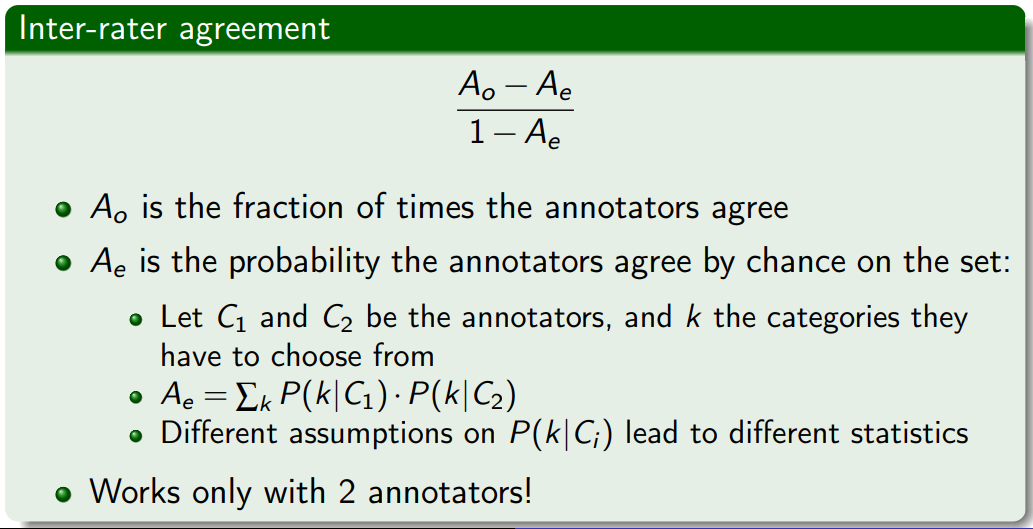
\includegraphics[width=0.5\linewidth]{internotersagreement.PNG}
    \caption{Formula per Agreement (A)}
    \label{fig:enter-label}
\end{figure}

Un modello è qualcosa che non esiste in natura costruito sulla realtà per fare delle predizioni; è un costrutto con cui noi esseri umani rappresentiamo il linguaggio, ad esempio un albero sintattico. Ma come ne giudichiamo la 'bontà'?

Consideriamo due o più persone (annotators) che si occupano di uno specifico task (linguistic) per testare il modello indipendentemente, se sono in accordo, allora questo potrebbe significare che il modello è simile alla rappresentazione del linguaggio che le persone hanno in mente. Come misuriamo il grado di agreement?

\end{abstract}

\section{Misurare la qualità di un sistema}
\begin{abstract}
Dati due sistemi S1 ed S2, vogliamo valutare la somiglianza fra i due, se sono effettivamente lo stesso sistema o meno.
I sistemi ricevono un determinato input C e formulano un risultato, un output simile implica che i due sistemi siano simili? Affichè le differenze rilevate siano statisticamente rilevanti, dobbiamo introdurre dei test significativi: \textbf{hypothesis tests}.

Ipotesi Nulla: H0:= le due distribuzioni sono uguali.
Ipotesi alternativa: Ha:= le due distribuzioni sono diverse.

Determinata l'ipotesi nulla cerchiamo di confutarla, impostando una soglia minima di verità (:= intervallo di confidenza).
Le procedure che si occupano di restituire la probabilità con cui l'ipotesi nulla viene rifiutata sono significance tests, di seguito riportiamo gli esempi di test presentati a lezione, tutti applicati al caso .

    \subsection{Sign Test}
    Supponiamo i due sistemi siano modelli di machine learning che vengono valutati sulla metrica di accuracy, su un determinato test set, o meglio, raccogliamo le accuracy dei sistemi per k volte, su batches differenti. (vabbe avete capito, tipo k-fold)
    S1: + + + + - - + - + -
    S2: - - - - + + - + - +
    E conservo il segno della differenza fra le due accuracy. Anche in questo caso affinchè i valori siano statistiche significativi è preferibile applicare tecniche stile bagging andando a simulare più batches.
    \subsection{Wilcoxon Test}
    Non l'ho capito molto bene e non so neanche se è stato fatto quest'anno, non credo.
    \subsection{Yeh (2000)}
    Considero un terzo sistema O, oracolo. anche qua non ho molti appunti.

\end{abstract}

